\chapter{Introduction}
\label{chap:QCD_low}

\section{Quantum Chromodynamic field theory}
	\subsection*{QCD Lagrangian}
	Following the same ideas of the localization of the initially global gauge transformation as it was employed for U(1) group transformation in QED \cite{opac-b1131978}, as a starting point one can write down the Lagrangian of femionic field $q(x)$ with mass parameter $m$:
	\beqa
		\mathcal{L}_{fermions} = \sum_i^{N_c,N_f} \bar{q}_i(i\dslash - m )q_i \;,
		\label{qcd_low:L_init}
	\eeqa
	Here we consider the Dirac fermionic field $q(x)$ in a fundamental representation of the color group SU(3), which is \textit{non-commutative} in nature and therefore  its semi-simple Lie algebra shall be considered. Thus the fermion field $q(x)$ has a $N_c=3$ color and $N_f=6$ flavor components $q_i(x), \; i=1,..,18$, where $i$ corresponds to super-index of color and flavor. Due to the gauge principle, we impose that the Lagrangian of the free Dirac field must be invariant under the SU(3) group transformation:
	\beqa
		\label{qcd_low:color_transform_ferm}
		q_i(x)\rightarrow  q_i^\prime(x)=U_{ij}q_i(x), \;\; U = \text{exp}(-it^a\theta^a) \;,
	\eeqa
	here $\theta^a$ are \textit{global} arbitrary parameters, independent of $x$ and $t^a, \; a=1,..,N^2_c-1$, are the generators associated to the used SU(3) group. Those can be expressed as $t^a=\lambda^2/2$, where $\lambda^a$ are Gell-Mann matrices, the standard choice of basis. The generators $t^a$ obey the Lie algebra:
	\beqa
		\label{qcd_low:commut_relation}
		[t^a,t^b]=if^{abc}t^c \;,
	\eeqa
	where $f^{abc}$ is totally antisymmetric structure function, specifying the group algebra. 
	\\
	The Lagrangian of fermions $\mathcal{L}_{fermions}$, given in Eq.(\ref{qcd_low:L_init}), is completely invariant under the global group transformation \Eq{\ref{qcd_low:color_transform_ferm}}. But after the localization of the transformation, the $\theta^a\rightarrow \theta^a(x)$ are \textit{local}, however, the $\mathcal{L}_{fermions}$ is no longer invariant because the derivative term would act now on $\theta^a(x)$ as well. Further, still it can be made independent, although it require to redefine the derivative to the covariant one:
	\beqa
		\partial_\mu \rightarrow D_\mu = \partial_\mu - ig t^a A^a_\mu \; ,
	\eeqa
	where $A^a_\mu$ are $N_c^2-1$ vector gauge fields, namely gluons, and $g$ is the coupling constant between $q$  and $A^a_\mu$. After this change and ommiting $i$ super-index the Lagrangian $\mathcal{L}_{fermions}$ is:
	\beqa
		\label{qcd_low:L_fermions}
		\mathcal{L}_{fermions} = \bar{q}(i\Dslash - m )q \;,
	\eeqa
	The given Lagrangian is is invariant under \Eq{\ref{qcd_low:color_transform_ferm}} color transformation, if the $A^a_\mu(x)$ obey the transformation rule:
	\beqa
		\label{qcd_low:color_transform_vector}
		t^a A^a_\mu \rightarrow t^a A^{\prime a}_\mu U\left( t^a A^a_\mu - \frac{i}{g}U^{-1}\partial_\mu U \right) U^{-1} \;,
	\eeqa
	in case of infinitesimal transformation $U(x)\approx 1- it^a\theta^a(x)$, also using the commutation relations \Eq{\ref{qcd_low:commut_relation}}, the \Eq{\ref{qcd_low:color_transform_vector}} becomes:
	\beqa
	\delta A^{\prime a}_\mu \rightarrow A^a_\mu + f^{abc}\theta^b A^c_\mu \frac{1}{g}\partial_\mu \theta^a \;,
	\eeqa
	As the infinitesimal transformation rule for $A^a_\mu$ contain the structure function $f^{abc}$, the gauge fields $A^a_\mu$ belong to the adjoint representation of the algebra of $SU(3)$. \\
	
	In the Lagrangian \Eq{\ref{qcd_low:L_fermions}} the fermion fields $q(x)$ interacts with the gauge field $A^a_\mu$, but in order to have a proper theory one need to specify a kinetic term for fields $A^a_\mu$. In order to do so, we need to find a right view of the gauge energy-impulse tensor, since the form $F^{a\mu\nu}F^a_{\mu\nu}$, with $F^a_{\mu\nu} = \partial_\mu A^a_\nu - \partial_\nu A^a_\mu$, is no longer invariant in respect to \Eq{\ref{qcd_low:color_transform_vector}} due to the non-Abelian nature of the color group $SU(3)$. Following ideas of electrodynamics, we derive the commutator of covariant derivatives to find:
	\beqa
		[D_\mu,D_\nu]=-igt^aF^a_{\mu\nu} \;,
	\eeqa	
	where $F^a_{\mu\nu} = \partial_\mu A^a_\nu - \partial_\nu A^a_\mu + gf^{abc}A^b_\mu A^c_\nu$ is the energy-impulse tensor for non-Abelian gauge fields $A^a_\mu$ of the group $SU(3)$, such as $F^{a\mu\nu}F^a_{\mu\nu}$ is gauge invariant. Conventionally normalized, it can be added to the Lagrangian \Eq{\ref{qcd_low:L_fermions}}. Thus, the general form of the Lagrangian of QCD invariant under the non-Abelian gauge transformation of the group $SU(3)$ is:
	\beqa
		\label{qcd_low:L_QCD}
		\mathcal{L}_{fermions} =\bar{q}(x)(i\gamma_\mu D^\mu - m_k )q(x) - \frac{1}{4}F^{a\mu\nu}F_{a\mu\nu} \;
	\eeqa
	There is a remarkable consequence of non-Abelian nature of $SU(3)$. Due to the term $gf^{abc}A^{b\mu}A^{c\nu}$ in $F^{a\mu\nu}$, there is a self-interaction amongst the gauge fields $A^{a\mu}$, leading to cubic and quartic terms. This is the crucial point in comparison to QED, the self-interaction of gluons is the main source of asymptotic freedom \cite{Gross:1973ju} and probably confinement. 
	
	\subsection*{The generating functional of QCD}
	In the previous section the classical Lagrangian of QCD \Eq{\ref{qcd_low:L_QCD}} was constructed. The next logical step is to quantize this classical theory. At this point we are working in Minkowski space-time.\\
	
	So far there are two well-known quantisation procedures. In the canonical approach to quantization of field theories, the fields treated as operators and their commutation relations should be defined. Then the Green's functions, the correlation functions, are calculated as vacuum expectation values of the time-ordered product of field operators. From another side, in the functional integral approach, fields are c-numbered functions of coordinate and the Lagrangian is given in a classical form. Since the path-integral approach is known to be the most robust technique to derive the \DS ,we will focus on this formalism.   \\

Any quantum field theory is completely defined by its Green's functions, which are then obtained by integrating the fields over all their functional forms with a suitable weight. As a starting point, the free scalar field $\phi(x)$ is considered, the n-point Green's function of this field are given as a time-ordered product of $n$ such fields: 
	\beqa
		\label{qcd_low:Green_func}
		\langle 0 | T[\hat{\phi(x_1)} ... \hat \phi(x_n) ] | 0 \rangle  = \frac{\int \mathcal{D} \phi \phi(x_1)...\phi(x_n)\; \text{exp}(iS) }{\int \mathcal{D}  \phi \; \text{exp}(iS) }
	\eeqa
where $S=\int dx^4( \mathcal{L} )$ is a classical action. However the \Eq{\ref{qcd_low:Green_func}} can be rewritten in a more convenient form of the generating functional, introducing the $J$ as a source fields:
    \beqa
        \label{qcd_low:Gen_functional_scal}
        \mathcal{Z} [J(x)] = \int \mathcal{D} \phi \; \text{exp} \left\lbrace i \int dx^4 ( \mathcal{L}  + J\phi)\right\rbrace 
    \eeqa
In this case the n-th Green's function can be obtained by taking appropriate number of functional derivatives with respect to the source $J$. 
    \beqa
        \langle 0 |T[\hat \phi(x_1)... \hat \phi(x_n) ]|0 \rangle = \frac{(-i)^n}{ \mathcal{Z}} \frac{\delta^n \mathcal{Z(J)} }{\delta J(x_1)...\delta J(x_n)} \vert_{J=0}
   \eeqa
For the gauge fields, the generating functional looks:
    \beqa
    	\label{qcd_low:Gen_functional_vec}
        \mathcal{Z}[J(x)] = \int \mathcal{D} A \; \text{exp} \left\lbrace i \int dx^4 ( \mathcal{L}  + J^\mu A_\mu )\right\rbrace 
    \eeqa
Although the source term $A^a_\mu J^{a \mu}$ is not gauge invariant, the physical predictions obtained within $\mathcal{Z}[J(x)]$ must be gauge independent. \\

Once we attempt to quantize given Lagrangian \Eq{\ref{qcd_low:Gen_functional_vec}} we face the uncertainty associated with the freedom of gauge. This can be clearly seen if set $J=0$. In this case the \Eq{\ref{qcd_low:Gen_functional_vec}} is given by:
	\beqa
		\label{qcd_low:Gen_functional_vec_0}
		\mathcal{Z}[0] = \int \mathcal{D} A\; \text{exp}( iS )
	\eeqa	
Since the action $S$ is invariant under gauge transformations $A^a_\mu \rightarrow A^{(\theta)a}_\mu$, we can generate a continuous infinity of $A^{(\theta)a}_\mu$ field configurations where the action $S$ is the same constant. Hence such functional integral is strongly divergent, as it is integrated over physically equivalent field configurations. In order to obtain physically meaningful results, one has to isolate the part of the functional integral, which counts each physical configuration only once. This can be achieved by setting restrictions upon the $A^a_\mu$, such as:
	\beqa
		\label{qcd_low:gauge_fix}
		G^\mu A^a_\mu = B^a
	\eeqa
To incorporate this constraint \Eq{\ref{qcd_low:gauge_fix}} in the functional integral \Eq{\ref{qcd_low:Gen_functional_vec_0}}, one need to inset the unity, given by Feddeev and Popov \cite{Faddeev196729}:
	\beqa
		\label{qcd_low:FP_unity}
		1 = \int \mathcal{D}[\theta(x)] \delta(G^\mu A^a_\mu - B^a) \; \text{det} M_G \;, \\ 
		\notag \text{where} \;\;\; (M_G(x,y))^{ab}= \left( \frac{\delta(G^\mu A^{(\theta) a}_\mu(x)}{\delta \theta^b(y)} \right)\;.
	\eeqa
Inserting \Eq{\ref{qcd_low:FP_unity}} into \Eq{\ref{qcd_low:Gen_functional_vec_0}} we find:
	\beqa
		\label{qcd_low:Gen_functional_vec_1}
		\mathcal{Z}[0] = \int \mathcal{D} [A] \; \text{det} M_G \int \prod_{a,x} \mathcal{D}[\theta^a(x)] \delta(G^\mu A^{(\theta) a}_\mu(x) - B^a)  \; \text{exp} \left\lbrace iS\right\rbrace 
	\eeqa
The delta function can be removed, by integrating $\mathcal{Z}[J(x)]$ over auxiliary field $B^a$ with a appropriate weight, given by Gaussian form $\text{exp} \left\lbrace  \frac{-i}{2\xi}\int d^4x (B^a(x))^2 \right\rbrace $, where $\xi$ is the gauge parameter. After that the integrand is independent of the group parameters $\theta^a(x)$ and therefore one can factor out the contribution of the $\int \prod_{a,x} \mathcal{D}[\theta^a(x)]$, which is infinite and will be cancelled out in the computation of Green's functions in \Eq{\ref{qcd_low:Green_func}}. Thus the generating functional takes a form:
	\beqa
		\label{qcd_low:Gen_functional_vec_2}
		\mathcal{Z}[J(x)] = \int \mathcal{D} [A] \; \text{det} M_G \; \text{exp}  \left\lbrace i \int d^4x \left( \mathcal{L} - \frac{1}{2\xi}(G^\mu A^a_\mu)^2 + J^{a\mu} A^a_\mu \right)  \right\rbrace \;\;
	\eeqa
	Choosing $G^\mu = \partial^\mu$ will correspond to Lorenz covariant gauges, which we will employ in this thesis and: 
	\beqa
		\label{qcd_low:Gauge_matrix}
		(M_G(x,y))^{ab} = -\frac{1}{g}(\delta^{ab}\partial^2 - g f^{abc}\partial^\mu A_\mu^c)\delta^4(x-y)
	\eeqa
	Note that in case of Abelian gauge theories the $f^{abc}=0$, and $M_G$ is independent of the gauge fields. Now it is easy to include fermions fields into the generating functional \Eq{\ref{qcd_low:Gen_functional_vec_2}}:
	\beqa
		\label{qcd_low:Gen_functional_vec_fer}
		\mathcal{Z}[J,\bar \eta, \eta] = \int \mathcal{D} [A \bar q q] \; \text{det} M_G \; \text{exp}  \left\lbrace i \int d^4x \left( \mathcal{L}_{eff} + J^{a\mu} A^a_\mu + \bar q \eta + \bar \eta q \right)  \right\rbrace \;\; \\
		\mathcal{L}_{eff} = \mathcal{L}_{QCD} - \frac{1}{2\xi}(G^\mu A^a_\mu)^2 \;. \;\;\;\;\;\;\;\;\;\;\;\;\;\;\;\;\;\;\;\;\;\;\;\;\;\;\;\;\;\;\;\;\;\;\;\;
	\eeqa
	Here $\eta$ and $\bar \eta$ are anti-commuting sources for the quark fields $q$ and $\bar q$, the $\mathcal{L}_{QCD}$ is given by \Eq{\ref{qcd_low:L_QCD}}. \\
	
	It is possible to exponentiate $\text{det} M_G$, in a same way as the gauge fixing condition, in order to incorporate it into effective Lagrangian. According to Faddeev and Popov \cite{Faddeev196729}, one can represent $\text{det} M_G$ as a integral over fictitious anti-commuting fields $\chi^a(x)$, so-called Feddeev-Popov ghosts:
	\beqa
	\label{qcd_low:FP_ghosts}
		\text{det} M_G = \int \mathcal{D} [\chi \chi^*]  \; \text{exp} \left\lbrace -i \int d^4x d^4y \chi^{a*}(x) (M_G(x,y))^{ab} \chi^b(y) \right\rbrace \;,
	\eeqa
where $M_G$ is given by \Eq{\ref{qcd_low:Gauge_matrix}}. The $\chi^a(x)$ is a complex field, obeying the Grassmann algebra and transforming under the adjoint representation of the non-Abelian gauge group. This is not a physical particle, since the spin and statistic of its quantum excitations have a wrong relation. Also according to Becchi, Rouet and Stora \cite{Becchi1976287} a certain connection between ghost fields $\chi, \chi^*$ and gauge parameter $\theta(x)$ can be established. The ghost action can be simplified by an integration by parts, such that:
	\beqa
		\label{qcd_low:FP_ghosts_action}
		\int d^4x d^4y \chi^{a*}(x) (M_G(x,y))^{ab} \chi^b(y) = - \int d^4x (\partial^\mu \chi^a(x))^* D^{ab}_\mu \chi^b(x) \;,
	\eeqa
where $D^{ab}_\mu = \delta^{ab}\partial_\mu - gf^{abc}A^c_\mu$ is the covariant derivative in adjoint representation. Inserting \Eq{\ref{qcd_low:FP_ghosts}} with the ghost action from \Eq{\ref{qcd_low:FP_ghosts_action}} into \Eq{\ref{qcd_low:Gen_functional_vec_fer}} we obtain the full generating functional of QCD:
	\beqa
		\label{qcd_low:Gen_functional_QCD}
		\mathcal{Z}[J,\bar \eta, \eta, \zeta, \zeta^*] = \int \mathcal{D} [A \bar q q \chi \chi^*] \; \text{exp}  \left\lbrace i \int d^4x \left( \mathcal{L}_{QCD} + \text{Sources} \right)  \right\rbrace \;,\; \\
	\notag	\mathcal{L}_{QCD} = \mathcal{L}_{Gluon} + \mathcal{L}_{Gauge\;fixing} + \mathcal{L}_{Quarks} + \mathcal{L}_{Ghosts}  \;, \;\;\;\;\;\;\;\;\;\;\; \\
	\notag \text{Sources} = J^{a\mu} A^a_\mu + \bar q \eta + \bar \eta q + \chi^{a*} \zeta^a + \zeta^{a*} \chi^a \;. \;\;\;\;\;\;\;\;\;\;\;\;\;
	\eeqa
Here $\zeta^{a*}$ and $\zeta^{a}$ are Grassmann-valued sources for the ghost fields. The $\mathcal{L}_{QCD}$ components given by:
	\beqa
		\mathcal{L}_{Gluon} = - \frac{1}{4}F^{a\mu\nu}F_{a\mu\nu} \;, \;\;\;\;\;\;\;\;\;\;\;\;\;\;\;\;\;\;\;\;\; \mathcal{L}_{Gauge\;fixing} = - \frac{1}{2\xi}(G^\mu A^a_\mu)^2 \;, \;\; \\
		\mathcal{L}_{Quarks} = \sum^{N_f}_k \bar{q_k}(i\gamma_\mu D^\mu - m_k )q_k \;, \;\;\;\;\; \mathcal{L}_{Ghosts} = (\partial^\mu \chi^a(x))^* D^{ab}_\mu \chi^b(x) \;.
	\eeqa
\section{Symmetries of QCD}
	On top of aforementioned local gauge color group $SU(3)_c$ and Lorenz invariance, there are a number of discrete symmetries, which the Lagrangian of Quantum Chromodynamics possess. %For a detailed account of QCD symmetries, see \cite{--}. 
	\subsection*{Chiral symmetry}
	Among those, the most important one is chiral symmetry, the symmetry of QCD in the limit of quark masses taken to zero. The dynamical spontaneous breaking of this symmetry generates mass for almost 95\% of the visible matter in the universe.   \\
	
	To set off, consider the light quark part of QCD Lagrangian \Eq{\ref{qcd_low:L_QCD}} with the quark mass matrix set to zero $m=0$. One can assume so since the current masses of the light $u,d$ quark are small enough ($\approx 5$ MeV) in comparison to the mass scale of hadrons, so that chiral symmetry is an approximate symmetry of the strong interactions. In this case the Lagrangian takes the form:
	\beqa
		\label{qcd_low:L_QCD_chiral}
		\mathcal{L}_{u,d} =\bar{q}(i\gamma_\mu D^\mu)q
	\eeqa	
	In order to make the symmetries more apparent we introduce the left- and right-handed projectors:
	\beqa
		P_L = \frac{1}{2}(1-\gamma_5) \;, \;\;\;\;\;\;\;\;\;\;\;\; P_R = \frac{1}{2}(1+\gamma_5)
	\eeqa
	Now we can decompose the quark fields into left- and right-handed components, $q_L = P_L q$ and $q_R = P_R q$. The \Eq{\ref{qcd_low:L_QCD_chiral}} afterwards becomes:
	\beqa
		\label{qcd_low:L_QCD_chiral_RL}
		\mathcal{L}_{u,d} = \bar{q_L}(i\gamma_\mu D^\mu)q_L +\bar{q_R}(i\gamma_\mu D^\mu)q_R
	\eeqa
	It is  apparent that there is no term that would connect left- and right-handed quark fields, therefore overall the Lagrangian is invariant under $U(2)$ transformation, namely $q^\prime \rightarrow \text{exp}(\alpha_i \sigma_i) q$, for each left- and right-handed quark. Here the $\sigma^i$ are the Pauli matrices. Hence the \Eq{\ref{qcd_low:L_QCD_chiral_RL}} yields a $U(2)_L \times U(2)_R = SU(2)_V \times SU(2)_A \times U(1)_V \times U(1)_A$ chiral symmetry, providing following Noether currents:
	\beqa
		\label{qcd_low:Noether_currents}
		&J^k_\mu = \bar{q}\gamma_{\mu}\sigma^k q \\
		&J^k_{5\mu} = \bar{q}\gamma_5\gamma_{\mu}\sigma^k q\\
		&J_\mu = \bar{q}\gamma_{\mu} q\\ 
		&J_{5\mu} = \bar{q}\gamma_5\gamma_{\mu} q\\ 
	\eeqa
Note that considering strange quark to be massless as well would extent this symmetry to $SU(3)_{\chi}$ chiral. \\

\vspace{-0.5cm}
However the experimental spectrum of QCD indicates, that the chiral symmetry is \textit{spontaneously broken} and the only symmetry is left is $U(1)_V \times SU(2)_V$. If it is so, according to Goldstone theorem, the theory must contain Goldstone bosons, massless spin-zero particles, and the number of these new degrees of freedom is equal to a number of generators of the broken symmetry. Particularly the spontaneous symmetry breaking $SU(2) \rightarrow SU(2)_V$ generates a triplet of pseudoscalar bosons, pions $(\pi^+, \pi^0, \pi^-)$. 
	
	The aforementioned chiral symmetry is of great importance for a low energy QCD physics, since the spontaneous breaking of this is the source of $95\%$ percent of hadrons mass. We will face this symmetry once more at the discussion of the chiral condensate.
	\subsection*{Axial symmetry}
	One may notice that, in addition to pion triplet given by $SU(2)_A$ breaking, the theory must contain one more Goldstone boson, associated with $U(1)_A$ broken symmetry. Using chiral perturbation theory, Weinberg \cite{PhysRevD.11.3583} estimated
the mass to be less than $\sqrt{3}m_\pi$. Among the known hadrons, the only candidates with the right quantum numbers are $\eta$(548) and $\eta^{\prime}$(958). Both violate the Weinberg bound. In fact, the $J_5$ current is not conserved at the quantum level due to the QCD axial anomaly:
\beqa
	\partial_\mu J^\mu_5 = \frac{g^2}{16\pi^2}F^{a\mu\nu}F_{a\mu\nu} = \frac{g^2}{16\pi^2}\partial_\mu \raisebox{2pt}{$\chi$}^\mu
\eeqa
And the topological charge given by:
\beqa
	Q_5 = \int d^3x \left[ q^\dagger \gamma_5 q - \frac{g^2}{16\pi^2} \in \raisebox{2pt}{$\chi$}^\mu \right] 
\eeqa
The existence of the topological charge $Q_5$ produce the non-zero topological susceptibility $\chi^2$, which can be related to additive anomaly mass correction via Witten-Veneziano formula \cite{Witten1979269,Veneziano1979213}:
\beqa
	m^2_A = 2\frac{N_f}{f_0^2}\chi^2
\eeqa


\section{Aspects of QCD}
	\subsection*{Confinement}
The most distinctive feature of the QCD theory, in comparison to QED, is that the basic blocks of it, like quark and gluons, are completely obscured to direct detection. All efforts done in the search of free quarks, even on the Moon surface, were unsuccessful. This stays not only for quarks and gluons, but also for any coloured states that can be made out of those. Such non-perturbative phenomenon is called \textit{colour confinement} and its  underlying origin is still not completely understood. Over the years several different pictures of confinement were developed, succeeding to explain various aspects of it; for a introductory review see \cite{Greensite201101}. 

The easiest and most straightforward model is the string model of confinement. It states that color electric flux between two color charged fermions forms a tube or a string, unlike the electric flux is being spread out. This string behaves at a long range scale as it has a constant tension $\sigma$, like naive Hooke's force law. However, due to a behaviour of QCD running coupling, at very short distances the interaction between quarks dominated by electric Coulomb potential. The incorporation of both aspects gives a rise to Cornell potential: $V(r) = - \frac{e}{r} + \sigma r$.
\begin{figure*}[t]
\tiny
 \begin{center}
  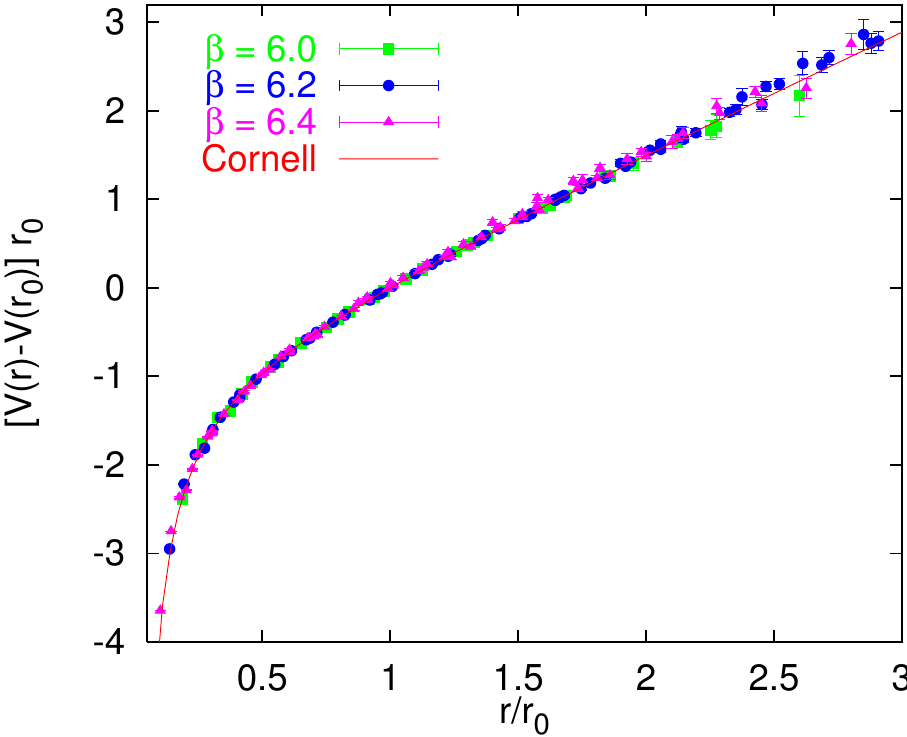
\includegraphics[width=0.45\textwidth]{figures/cornell_V.png}
 \end{center}
 \caption{\footnotesize Cornell potential compared to quenched $SU_c(3)$ potential, taken from \cite{Bali:2000gf}. The $r$ is a distance between quarks.}\label{fig:cornell_V} 
\end{figure*}
It is clear that a potential energy increases as two quarks are being pull apart, although when the energy is bigger than that of meson mass, the string breaks into two mesons.

A more recent picture of the QCD confinement comes from lattice simulations, where the co-called center vortices play a major role. Center vortices are very specific objects carrying the topological charge, coming from central symmetry of the $SU_c(3)$. These vortices are of the great importance for lattice studies, since it was found that string tension vanishes at removal of central vortices, therefore providing a link between these two phenomena.

In case of \DS framework the confinement can be concluded from analytical structure of dressed quark propagator. The quark dressing functions posses complex conjugate poles, which lead to a violation of Osterwalder--Schrader axiom of reflection positivity \cite{Osterwalder:1973dx}, and therefore ensure that a quark is not a asymptotic physical state, \textit{i.e.}confined. Note however, that this result is truncation dependent.

	\subsection*{Chiral condensate}
Spontaneous chiral symmetry breaking is the phenomena that leads to a generation of non-vanishing ground state of QCD Lagrangian. To approach this problem consider the term $\langle0|\bar{q}q|0\rangle$ that connects right- and left-handed quark fields
\beqa
	\langle0|\bar{q}q|0\rangle = \langle0|\bar{q_R}q_L + \bar{q_L}q_R |0\rangle\;.
\eeqa
It is easy to show that a dynamic generation of such term breaks chiral symmetry, while keep being invariant under $SU(2)_V \times U(1)_V$. Formally this matrix element is defined as
\beqa
	\langle0|\bar{q}q|0\rangle = \int \frac{d^4k}{(2\pi)^4} Tr\left[  S(k) \right] \;.
\eeqa
In case of trivial vacuum the corresponding expectation value, which is called \textit{chiral condensate}, vanishes, $\langle0|\bar{q}q|0\rangle \equiv \langle\bar{q}q\rangle = 0$. However this is no longer true in case of non-perturbative vacuum of QCD, where the ground state is non-zero: $\langle0|\bar{q}q|0\rangle = \langle0|\bar{u}u + \bar{d}d|0\rangle \approx -(250 \; \text{MeV})^3$. On the propagator level this effect appears in quark mass function $M(p^2)$: in infra-red region the mass function is $M(0)\approx 400 \; MeV$, generating dynamically constituent quark mass. Since mesons and baryons are quark constructions this generates masses for them as well, except Goldstone pseusoscalar bosons, the pions, which stay massless.

However in the real world chiral symmetry is broken spontaneously and \textit{explicitly}. Explicit breaking is provided by interaction between quark fields and Higgs boson condensate, such as this produces small \textit{current} masses for $u,d$. In this case Goldstone pseusoscalar bosons are no longer massless and Gell-Mann, Oakes and Renner \cite{GellMann:1968rz} showed that the square of the mass of the Goldstone bosons grows in proportion to $m_u + m_d$
\beqa
	\label{qcd_low:GMOR}
	M^2_\pi = (m_u+m_d)\frac{\langle0|\bar{q}q|0\rangle}{f^2_\pi}
\eeqa

	\subsection*{Running coupling of QCD}
The renormalization group equation of QCD for a one-loop peturbation order $\beta$-function takes the following form:
\beqa
    \label{qcd_low:renorm_eq}
	\mu\frac{\partial\alpha_s}{\partial\mu}=-(11-\frac{2}{3}N_f)\frac{\alpha_s^2}{2\pi} \;,
\eeqa
where $\alpha_s$ is QCD running coupling, $\mu$ is the scale dependence parameter and $(11-\frac{2}{3}N_f) = \beta_0$ is a first non-vanishing term in $\beta$-function. The \Eq{\ref{qcd_low:renorm_eq}} can be solved, yielding the solution
\begin{figure*}[h]
 \begin{center}
  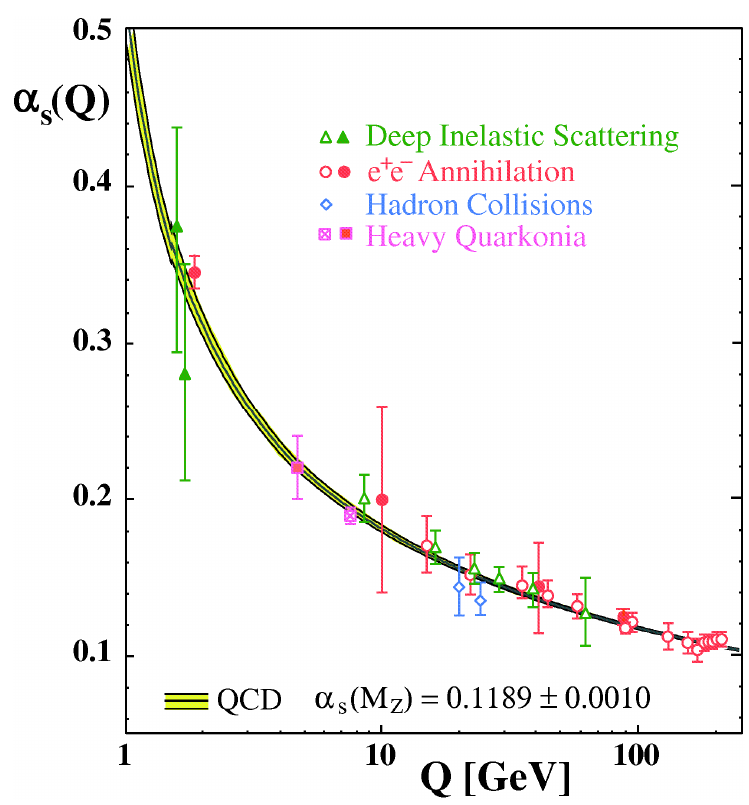
\includegraphics[width=0.55\textwidth]{figures/running_coupling2.png}
 \end{center}
 %\vspace{-1cm}
 \caption{\footnotesize 
% (b) The coupling constant for different lattice settings compared
%to perturbative expression plus power corrections in the high momenta region. (a) Region of small momenta
%is zoomed. Figire is taken from \cite{Boucaud:2002fx}.
Summary of measurements of $\alpha_s(Q)$ as a function of the respective energy scale $Q$.
The curves are the QCD predictions for the combined world average value of $\alpha_s(M_Z)$. Figure is taken from \cite{Bethke:2006ac}.
}
\label{fig:running_coupling} 
\end{figure*}
\beqa
	\alpha_s(Q^2) = \frac{4\pi}{\beta_0 ln(Q^2/\Lambda^2_{QCD})}\;.
\eeqa
This solution is valid only for $Q^2 >> \Lambda^2_{QCD}$, while the parameter $\Lambda^2_{QCD} \approx 230 \; \text{MeV}$ defines the energy scale,
below which the perturbation series break due to large running coupling $\alpha_s$. 

This is one of the facts that make unreachable all underlying physics of formation and structure of hadron to perturbative QCD theory, encouraging to develop non-perturbative approaches, such as: Lattice QCD, instanton liquid model, quark models, effective chiral Lagrangians, QCD sum rules and the one employed throughout this thesis - the \DS/\BS  functional method.

%\subsection*{Bound states in QCD}
%
%\begin{figure*}[h]
% \begin{center}
%  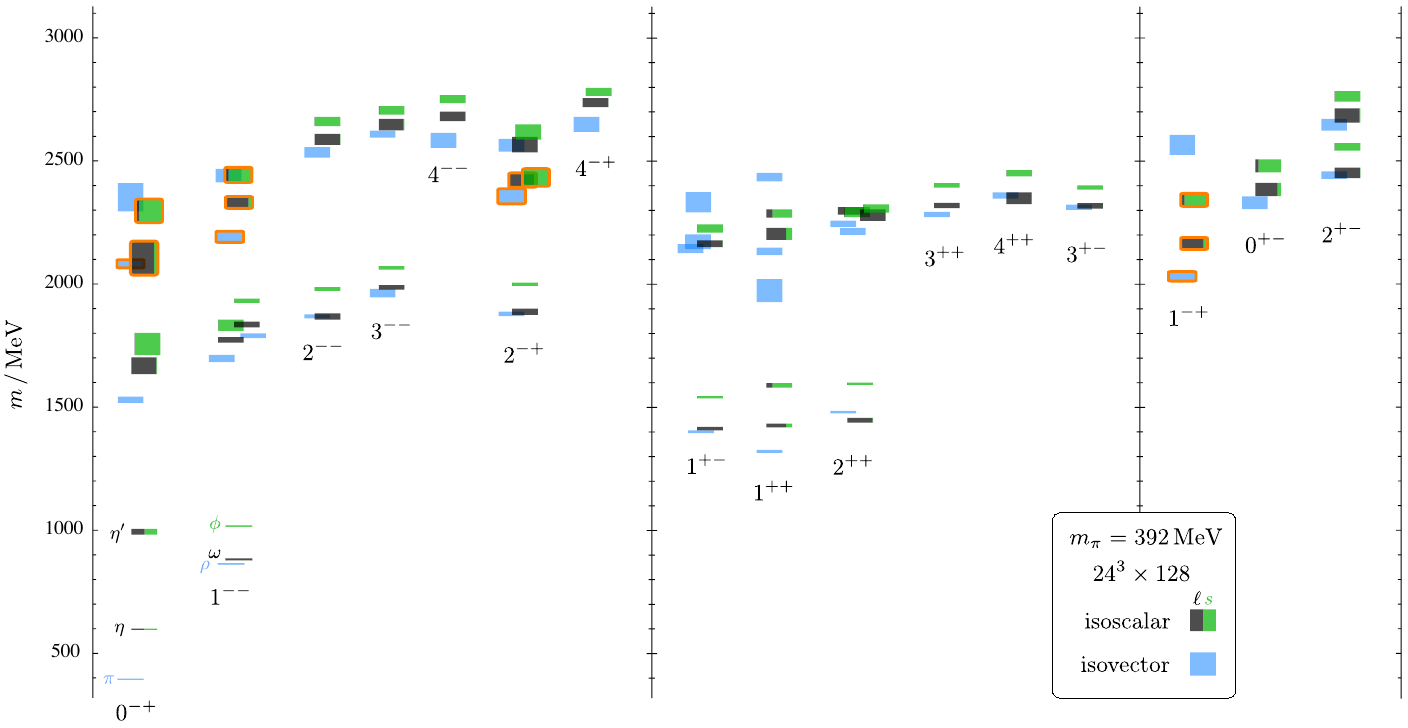
\includegraphics[width=0.99\textwidth]{figures/Lattice_spectra.png}
% \end{center}
% \caption{\footnotesize 
%Isoscalar (green/black) and isovector (blue) meson spectrum on the $m_\pi =$ 391 MeV, 243 $\times$ 128 lattice. The vertical
%height of each box indicates the statistical uncertainty on the mass determination. States outlined in orange are the lowest-lying
%states having dominant overlap with operators featuring a chromomagnetic construction. Figire is taken from \cite{Dudek:2013yja}.
%}
%\label{fig:running_coupling} 
%\end{figure*}
